The course first edition was coincidental with the outbreak of the SARS-CoV-2 pandemic.
Lockdowns forced us to implement emergency remote lessons based on digital teleconference software solutions.
The teaching staff having previously used Jupyter Notebooks at laboratory courses wrote the lessons for the first weeks taking advantage of Python code to perform the required calculations and also plotting its results.
While the first synchronical meeting was conducted, it was verified that each one of the students was sitted in front of a computer.
The opportunity to force students to use code to solve the exercises set was quickly grasped.
After an initial adaptation period, the students recognized the virtues of this methodology. 
Even assessments were more enriching than in a conventional course as it reached the complexity of simulating industrial-like mechanical systems.
During the four semesters when lessons were remote, adoption of asynchronous consultations grew.
As the lesson material was published in advance to the meetings, the teaching staff started to suggest that it be read before it in order to discuss it rather than present it.
This then led to suggest that some excercises be solved also in advance.
Gradually this led to free time at the meetings thus allowing the students to work on the excercises while they could make synchronical consultations on them to the staff.
By the time in person meetings at classrooms began, the staff decided to put to test a radical proposal: avoid giving lectures altogheter, switching to the \textit{flipped classroom} methodology \cite{oflaherty_use_2015, noauthor_flipped_2024} schematised in figure \ref{fig:flippedClassroomSchedule}.

\begin{figure}[ht]
\centering
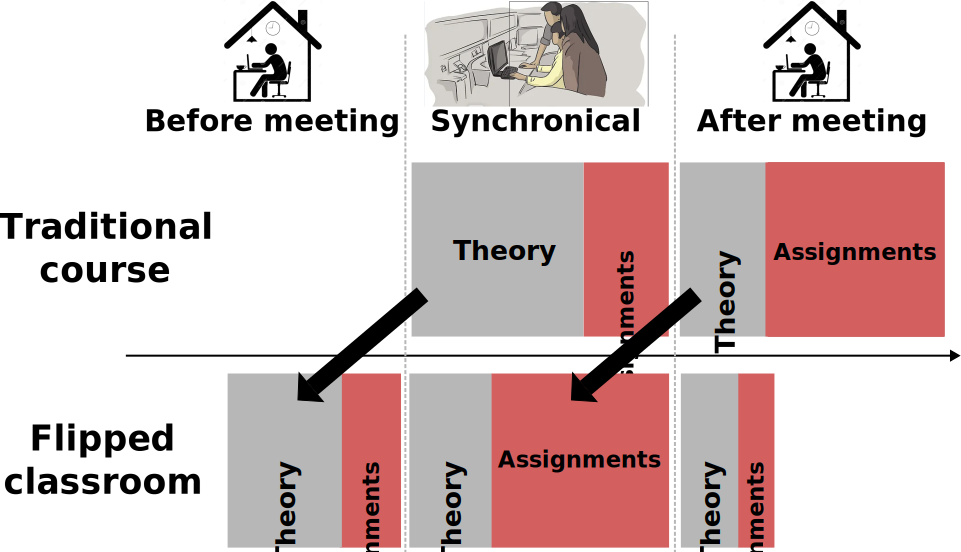
\includegraphics[width=0.9\linewidth]{figuras/flippedClassroomSchedule.pdf}
\caption{This schematizes how the student allocates the same amount of time in our flipped classroom course compared to a traditional one. There is a synchronic meeting for each thematic block. Reading theory and starting the work on their exercise set is mandatory before the meeting.}
\label{fig:flippedClassroomSchedule}
\end{figure}

The current course syllabus is strictly divided into weekly distinct thematic blocks with a single synchronic meeting devoted to it.
No lecturing occurs during the meeting, thus all the staff's available time is reserved for one to one consultations on the excercise sets.
If a single subject is perceived to need some review, a quick lecture on the particular is improvised based on the material at the repository.
Students are required to read in anticipation the respective material on theory published beforehand in the course repository as Jupyter Notebooks, alongside videos with discussions on important topics.
They also must begin working on the exercises before the meeting where they seek clarification on both, the theory and difficulties found while trying to solve the practice problems. 
As they finish up them in a later date and usually that requires some review on the theory, an asynchronic communication channel is available where the teaching staff can answer their questions on both matters.
